\documentclass[11pt,a4paper]{article}
\usepackage[utf8]{inputenc}
\usepackage[spanish,es-tabla]{babel}
\usepackage{amsmath}
\usepackage{amsfonts}
\usepackage{amssymb}
\usepackage{graphicx}

\usepackage{vmargin}

\setpapersize{A4}
\setmargins{2.5cm}              % margen izquierdo
{1.5cm}                         % margen superior
{16.5cm}                        % anchura del texto
{23.42cm}                       % altura del texto
{10pt}                          % altura de los encabezados
{1cm}                           % espacio entre el texto y los encabezados
{0pt}                           % altura del pie de página
{2cm}                           % espacio entre el texto y el pie de página

\title{ 
    Emisión de titulos universitarios
    en la Blockchain
}
\author{
    Saez, Lautaro Andres \\ \small{ LautaroAndresSaez@gmail.com } 
    \and 
    Riperto, Adriel Aaron \\ \small{ aaron.ariperto@gmail.com } 
}
\date{\today}

\begin{document}
    \maketitle

    \section{Introducción}

    \section{Estado del arte}

        Esta sección tiene como objetivo tratara el estado actual de la tematica a abordar.
        En general debido a que blockchain se encuentra en constante crecimiento, no hay 
        grandes aplicaciones implementadas en el ambito de titulos academicos, sino que existen
        trabajos que proponen modelos a implementar. %Correguir implementaciones!

        \subsection{Blockchain federal Argentina}

        En primer lugar desde la pagina web de la Blockchain federal  Argentina %Incluir referencia a la BFA 
        se menciona este trabajo como una posible aplicación nombrando las 
        ventajas que este tiene las cuales son:
        
        \begin{itemize}
            \item Garantiza que no sea posible alterar la 
            información de las actas sin que esa modificación sea detectada y así aumenta la confianza en la autenticidad de los títulos emitidos. 
            \item Transparencia en el proceso de digitalización.
            \item Permite un contexto de confianza entre organismos y partes interesadas. 
            \item Auditable.
            \item Permite demostrar que no existen actos de negligencia (títulos truchos) en torno a la emisión de títulos.
            \item Se podría dar diferentes vigencias a certificado de títulos en trámite, o similares, certificadas en la blockchain.
        \end{itemize}

        Por otro lado se proponen posibles mejoras a esta implementción creando un portafolios digital, lo cual 
        permitiria modificar los permisos de acceso.

        \begin{figure}
            \centering
            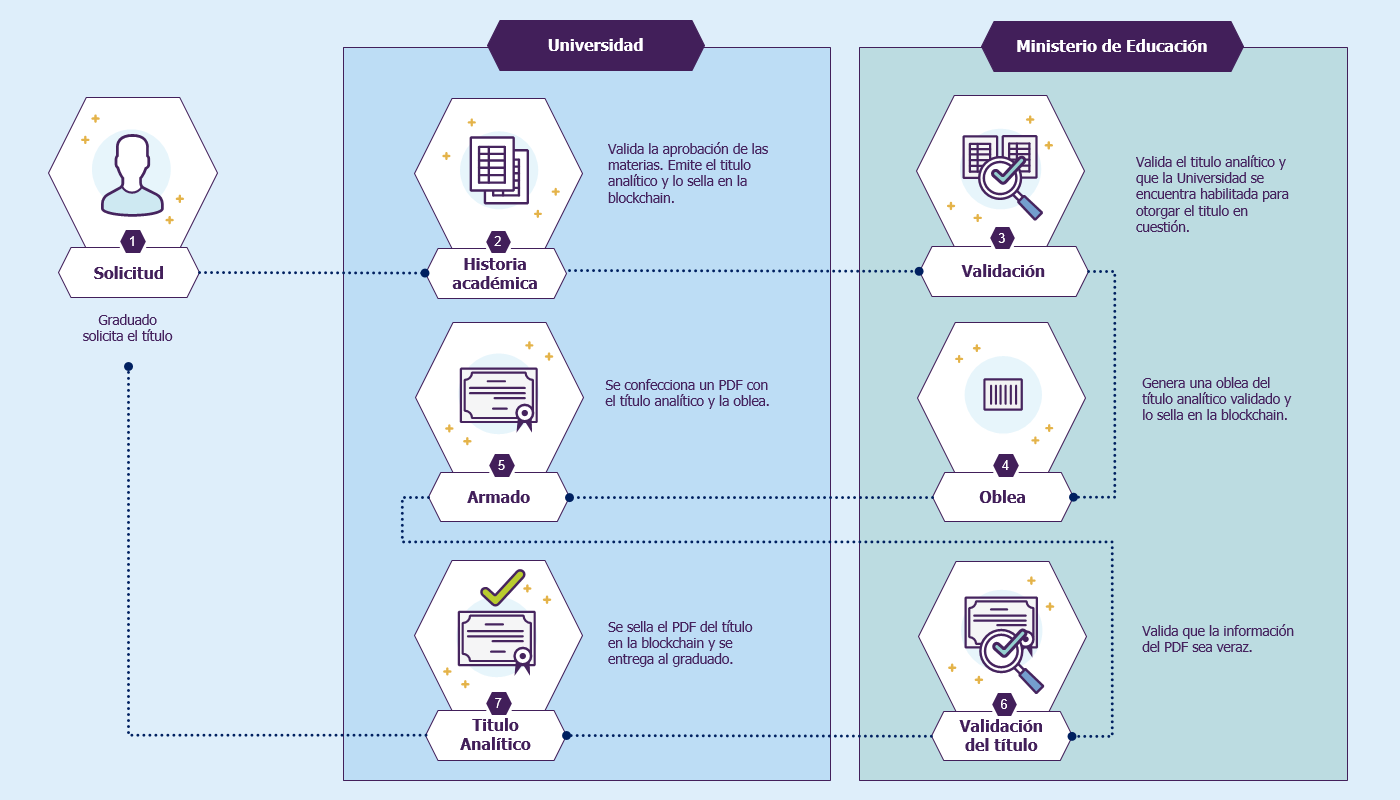
\includegraphics[width=\textwidth]{Img/cuadro_problematica.png}
            \caption{}
            \label{fig:cuadro_problematica}
        \end{figure}

        \subsection{AWS example}
    \section{Objetivos}

        En esta seccion se establecen los siguientes objetivos para el proyecto, 
        presentando posibles mejoras al mismo como objetivos opcionales.

        Los objetivos principales son:

        \begin{itemize}
            \item Realizar el backend de la aplicacion con Solidity.
            \item Realizar un deploy en la BFA.
            \item Crear una frontend en React.
        \end{itemize}

        Por otro lado se presentan las siguientes mejores:

        \begin{itemize}
            \item Crear una aplicacion para moviles utilizando React Native.
            \item Permitir llevar un control de las materias rendidas.
        \end{itemize}

        En la Figura \ref{fig:cuadro_problematica} se observa como se realiza una solicitud 
        del estado del titulo.
        
        \begin{figure}
            \centering
            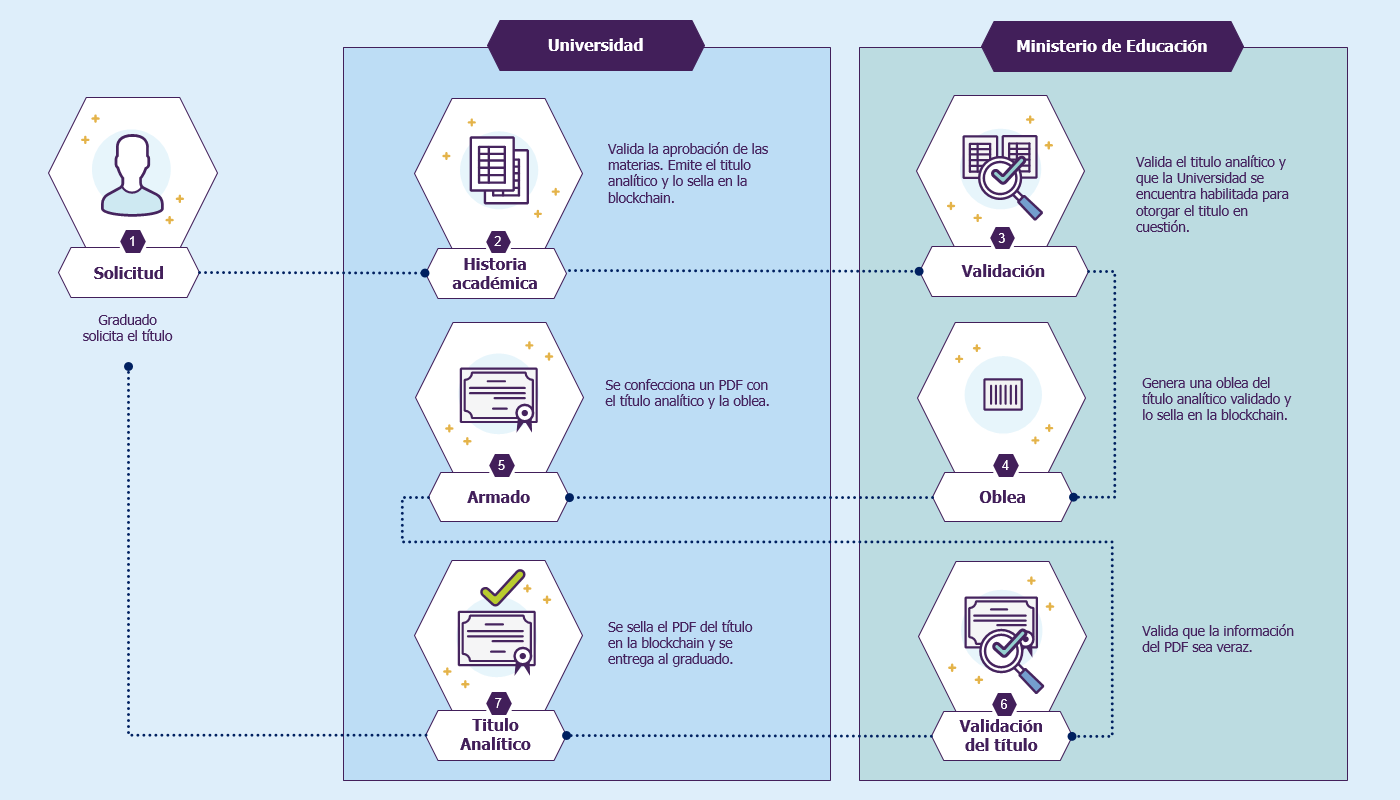
\includegraphics[width=\textwidth]{Img/cuadro_problematica.png}
            \caption{}
            \label{fig:cuadro_problematica}
        \end{figure}



    \section{Desafíos}

    \section{Etapas}

    \section{Conclusiones}

\end{document}